% Created 2017-04-19 Wed 08:01
% Intended LaTeX compiler: pdflatex
\documentclass[11pt]{article}
\usepackage[utf8]{inputenc}
\usepackage[T1]{fontenc}
\usepackage{graphicx}
\usepackage{grffile}
\usepackage{longtable}
\usepackage{wrapfig}
\usepackage{rotating}
\usepackage[normalem]{ulem}
\usepackage{amsmath}
\usepackage{textcomp}
\usepackage{amssymb}
\usepackage{capt-of}
\usepackage{hyperref}
\usepackage[margin=1.2in]{geometry}
\usepackage{setspace}
\onehalfspacing
\usepackage{parskip}
\usepackage{booktabs}
\newcommand{\pr}{\mathrm{Pr}}
\setcounter{secnumdepth}{2}
\author{Zheng Tian}
\date{}
\title{Replication of Examples in Chapter 6}
\hypersetup{
 pdfauthor={Zheng Tian},
 pdftitle={Replication of Examples in Chapter 6},
 pdfkeywords={},
 pdfsubject={},
 pdfcreator={Emacs 25.1.1 (Org mode 9.0.3)},
 pdflang={English}}
\begin{document}

\maketitle

\section{Introduction}
\label{sec:org453d38a}
This document is to show how to perform hypothesis testing for a
single coefficient in a simple linear regression model. I replicate
examples that occur in Chapter 6.

\section{Scatterplot with two regressors}
\label{sec:orgcc1fe7c}

\begin{verbatim}
library(AER)
library(foreign)
classdata <- read.dta("caschool.dta")
\end{verbatim}

We can draw the scatterplots of \emph{STR} against \emph{TestScr} and \emph{PctEl}
against \emph{TestScr}, and arrange the two scatterplot in one frame.

\begin{verbatim}
# scatterplot
oldpar <- par(mfrow = c(2, 1))

plot(classdata$str, classdata$testscr, col = "red",
    main = "student-teacher ratio vs test scores",
     xlab = "Student-teacher ratio", ylab = "Test scores")

plot(classdata$el_pct, classdata$testscr, col = "blue",
     main = "English learners vs test scores",
     xlab = "Percentage of English learners",
     ylab = "Test scores")

par(oldpar)
\end{verbatim}

\begin{figure}[htbp]
\centering
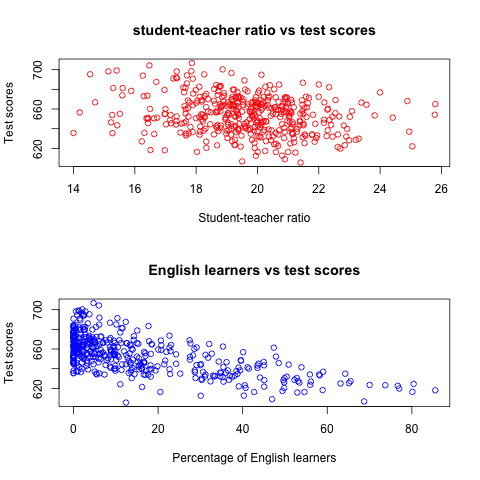
\includegraphics[width=0.9\textwidth]{./img/sp2.png}
\caption{The scatterplots of test scores against student-teacher ratios and the percentage of English learners}
\end{figure}

\section{The OLS estimation of the multiple regression model}
\label{sec:org8aaccd7}

The multiple regression model is
\begin{equation}
\label{eq:testscr-str-1}
TestScore_i = \beta_0 + \beta_1 STR_i + \beta_2 PctEL + u_i
\end{equation}

Then we define the \texttt{formula} object for the multiple regression
model and estimate it

\begin{verbatim}
mod1 <- lm(testscr ~ str + el_pct, data = classdata)
(sum.mod1 <- summary(mod1))
\end{verbatim}

\begin{verbatim}
Call:
lm(formula = testscr ~ str + el_pct, data = classdata)

Residuals:
    Min      1Q  Median      3Q     Max
-48.845 -10.240  -0.308   9.815  43.461

Coefficients:
             Estimate Std. Error t value Pr(>|t|)
(Intercept) 686.03225    7.41131  92.566  < 2e-16 ***
str          -1.10130    0.38028  -2.896  0.00398 **
el_pct       -0.64978    0.03934 -16.516  < 2e-16 ***
---
Signif. codes:  0 ‘***’ 0.001 ‘**’ 0.01 ‘*’ 0.05 ‘.’ 0.1 ‘ ’ 1

Residual standard error: 14.46 on 417 degrees of freedom
Multiple R-squared:  0.4264,	Adjusted R-squared:  0.4237
F-statistic:   155 on 2 and 417 DF,  p-value: < 2.2e-16
\end{verbatim}

We can get the estimated coefficients, predicted values, residuals,
SER, R\(^{\text{2}}\), and the adjusted R\(^{\text{2}}\) using the following commands.

\begin{verbatim}
# get the compoenents
b <- coef(mod1) # coefficients
y.hat <- predict(mod1) # predicted value of y
u.hat <- resid(mod1) # residuals
SER <- sum.mod1$sigma # standard error of regression
R2 <- sum.mod1$r.squared # R squared
AR2 <- sum.mod1$adj.r.squared # adjusted R squared
\end{verbatim}

So the coefficient on \emph{STR} is
\texttt{-1.101},
which means that, holding \emph{PctEL} constant, one unit increase in
\emph{STR} will lead to a decrease in \emph{TestScr} by
\texttt{-1.101} units.
The R\(^{\text{2}}\) and the adjusted R\(^{\text{2}}\) are round
\texttt{0.426}
and \texttt{0.424}, respectively.

The homoskedasticity-only covariance matrix and the
heteroskedasticity-consistent covariance matrix of the coefficients
can be computed by the command below
\begin{verbatim}
(vcov.hm <- vcov(mod1)) # homoskedasticity-only covariance matrix
se.hm <- sqrt(diag(vcov.hm)) # homoskedasticity-only standard error
\end{verbatim}

\begin{verbatim}
            (Intercept)         str       el_pct
(Intercept) 54.92755274 -2.79596671  0.030730824
str         -2.79596671  0.14461160 -0.002807340
el_pct       0.03073082 -0.00280734  0.001547836
\end{verbatim}

\begin{verbatim}
(vcov.ht <- vcovHC(mod1, type = "HC1")) # HCCM
se.ht <- sqrt(diag(vcov.ht)) # heterskedasticity-robust se
\end{verbatim}

\begin{verbatim}
            (Intercept)           str        el_pct
(Intercept) 76.18189018 -3.7569802107 -0.0134448546
str         -3.75698021  0.1873566583 -0.0003131024
el_pct      -0.01344485 -0.0003131024  0.0009629703
\end{verbatim}

\section{An illustration of \(TSS = ESS + SSR\)}
\label{sec:orgde6d73d}
Let's verify the property of the OLS estimator, \(TSS = ESS + SSR\). We
can compute the three quantities using the following commands.

\begin{verbatim}
TSS <- with(classdata, sum((testscr - mean(testscr))^2))
ESS <- sum((y.hat - mean(y.hat))^2)
SSR <- sum(u.hat^2)
\end{verbatim}

When we directly verify the equality, what we get is \texttt{FALSE}.
\begin{verbatim}
TSS == ESS + SSR
\end{verbatim}

\begin{verbatim}
[1] FALSE
\end{verbatim}

This is due to the error of computation with floating point
numbers. So instead of directly compare the LHS with the RHS, we can
do the following,
\begin{verbatim}
abs(TSS - ESS - SSR) < 1.0e-9
\end{verbatim}

\begin{verbatim}
[1] TRUE
\end{verbatim}

\section{An illustration of the FWL theorem}
\label{sec:orgbf33154}
Now let's demonstrate the FWL theorem. Suppose we are interested in
the effect of \emph{STR} on \emph{TestScr} controlling for \emph{PctEl}. So according
to the FWL theorem, we can follow three steps to estimate the
coefficient on \emph{STR}
\begin{description}
\item[{Step 1}] Regress \emph{STR} on \emph{PctEL} and get the residuals;
\item[{Step 2}] Regress \emph{TestScr} on \emph{PctEl} and get the residuals;
\item[{Step 3}] Regress the residuals in the second step on the residuals
in the first step to get the estimated coefficient.
\end{description}
These steps can be implemented by the following command
\begin{verbatim}
# step 1
m1 <- lm(str ~ el_pct, data = classdata)
# step 2
m2 <- lm(testscr ~ el_pct, data = classdata)
# step 3
m3 <- lm(resid(m2) ~ resid(m1) - 1)
\end{verbatim}

Finally, we compare the estimated coefficient on \emph{STR} following the
steps above and that estimated using both \emph{STR} and \emph{PctEl} at a
time.
\begin{verbatim}
abs(coef(m3) - b[2]) < 1.0e-10
\end{verbatim}

\begin{verbatim}
resid(m1)
     TRUE
\end{verbatim}

\section{An illustration of the dummy variable trap}
\label{sec:orgd71630a}
We define dummy variables for small class, medium class, large
class, according to \emph{STR}
\begin{equation*}
Small =
\begin{cases}
1,\; &\text{if } STR < 18 \\
0,\; &\text{otherwise } }
\end{cases},
Medium =
\begin{cases}
1,\; &\text{if } 18 \leq STR < 20 \\
0,\; &\text{otherwise } }
\end{cases},
Large =
\begin{cases}
1,\; &\text{if } STR \geq 20 \\
0,\; &\text{otherwise } }
\end{cases}
\end{equation*}

Defining these three dummy variables can be accomplished by the
following commands
\begin{verbatim}
small <- ifelse(classdata$str < 18, 1, 0)
middle <- ifelse(classdata$str >= 18 & classdata$str < 20, 1, 0)
large <- ifelse(classdata$str >= 20, 1, 0)
\end{verbatim}
from which we get three vectors consisting of 1 and 0.

We can more easily define dummy variables in R using a \texttt{factor}
object as follows
\begin{verbatim}
classsize <- ifelse(classdata$str < 18, "small",
	     ifelse(classdata$str >= 18 & classdata$str < 20, "medium", "large"))
classsize <- as.factor(classsize)
\end{verbatim}

Let's first try to estimate a model with an intercept and all three
dummy variables, which is an example of the dummy variable trap.
\begin{verbatim}
mod3 <- lm(testscr ~ small + middle + large, data = classdata)
summary(mod3)
\end{verbatim}

\begin{verbatim}
Call:
lm(formula = testscr ~ small + middle + large, data = classdata)

Residuals:
    Min      1Q  Median      3Q     Max
-48.441 -14.354   0.534  13.749  45.109

Coefficients: (1 not defined because of singularities)
            Estimate Std. Error t value Pr(>|t|)
(Intercept)  649.979      1.378 471.721  < 2e-16 ***
small         12.067      2.551   4.731 3.06e-06 ***
middle         5.212      2.005   2.600  0.00965 **
large             NA         NA      NA       NA
---
Signif. codes:  0 ‘***’ 0.001 ‘**’ 0.01 ‘*’ 0.05 ‘.’ 0.1 ‘ ’ 1

Residual standard error: 18.59 on 417 degrees of freedom
Multiple R-squared:  0.05272,	Adjusted R-squared:  0.04818
F-statistic:  11.6 on 2 and 417 DF,  p-value: 1.247e-05
\end{verbatim}

We can see that R automatically drop the dummy variable for large
classes in estimation, resulting in \texttt{NA} for \texttt{large} and a warning
message saying that \texttt{Coefficients: (1 not defined because of
singularities)}. So we should drop a dummy variable to set up a correct
model.

\begin{verbatim}
mod3.a <- lm(testscr ~ small + middle, data = classdata)
summary(mod3.a)
\end{verbatim}

\begin{verbatim}
Call:
lm(formula = testscr ~ small + middle, data = classdata)

Residuals:
    Min      1Q  Median      3Q     Max
-48.441 -14.354   0.534  13.749  45.109

Coefficients:
            Estimate Std. Error t value Pr(>|t|)
(Intercept)  649.979      1.378 471.721  < 2e-16 ***
small         12.067      2.551   4.731 3.06e-06 ***
middle         5.212      2.005   2.600  0.00965 **
---
Signif. codes:  0 ‘***’ 0.001 ‘**’ 0.01 ‘*’ 0.05 ‘.’ 0.1 ‘ ’ 1

Residual standard error: 18.59 on 417 degrees of freedom
Multiple R-squared:  0.05272,	Adjusted R-squared:  0.04818
F-statistic:  11.6 on 2 and 417 DF,  p-value: 1.247e-05
\end{verbatim}

Equivalently, we can drop the intercept term.
\begin{verbatim}
mod4 <- lm(testscr ~ small + middle + large - 1, data = classdata)
summary(mod4)
\end{verbatim}

\begin{verbatim}
Call:
lm(formula = testscr ~ small + middle + large - 1, data = classdata)

Residuals:
    Min      1Q  Median      3Q     Max
-48.441 -14.354   0.534  13.749  45.109

Coefficients:
       Estimate Std. Error t value Pr(>|t|)
small   662.046      2.146   308.4   <2e-16 ***
middle  655.191      1.456   450.0   <2e-16 ***
large   649.979      1.378   471.7   <2e-16 ***
---
Signif. codes:  0 ‘***’ 0.001 ‘**’ 0.01 ‘*’ 0.05 ‘.’ 0.1 ‘ ’ 1

Residual standard error: 18.59 on 417 degrees of freedom
Multiple R-squared:  0.9992,	Adjusted R-squared:  0.9992
F-statistic: 1.734e+05 on 3 and 417 DF,  p-value: < 2.2e-16
\end{verbatim}

In fact, when we use the \texttt{factor} object, \texttt{classsize}, the formula get
easier as follows,

\begin{verbatim}
mod5 <- lm(testscr ~ classsize, data = classdata)
summary(mod5)
\end{verbatim}

\begin{verbatim}
Call:
lm(formula = testscr ~ classsize, data = classdata)

Residuals:
    Min      1Q  Median      3Q     Max
-48.441 -14.354   0.534  13.749  45.109

Coefficients:
                Estimate Std. Error t value Pr(>|t|)
(Intercept)      649.979      1.378 471.721  < 2e-16 ***
classsizemedium    5.212      2.005   2.600  0.00965 **
classsizesmall    12.067      2.551   4.731 3.06e-06 ***
---
Signif. codes:  0 ‘***’ 0.001 ‘**’ 0.01 ‘*’ 0.05 ‘.’ 0.1 ‘ ’ 1

Residual standard error: 18.59 on 417 degrees of freedom
Multiple R-squared:  0.05272,	Adjusted R-squared:  0.04818
F-statistic:  11.6 on 2 and 417 DF,  p-value: 1.247e-05
\end{verbatim}

which yields the same estimation as specifying two dummy variables
explicitly.
\end{document}